\section{Example \textit{C} project}

\begin{frame}
    \frametitle{Example \textit{C} project}

    We are starting with an example \textit{C} project with \alert{multiple subdirectories} symbolizing a complex project structure. Each directory is responsible for a single binary. All besides the core functions should reside in the \texttt{lib} directory.

    \begin{figure}[H]
        \centering
        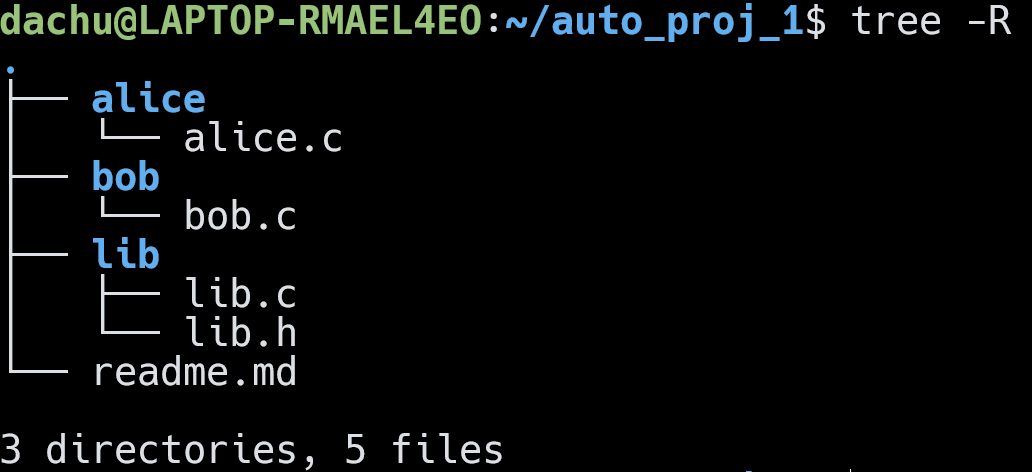
\includegraphics[width=0.8\textwidth]{../figure/init_state.png}
        \caption*{Tree structure of the example project.}
    \end{figure}
\end{frame}

% xxx move source files to script dir
% xxx remove initial commit

\begin{frame}
    \frametitle{lib/lib.c \& lib/lib.h}

    \begin{figure}[hp]
        \centering
        \hfill
        \begin{minipage}{.8\textwidth}
            \inputminted[
                mathescape,
                linenos,
                autogobble,
                fontsize=\scriptsize,
            ]{bash}{E:\\GitHub\\presentation_in_LaTeX\\c_project_development\\script\\lib.c}
        \end{minipage}
        \hfill
        \caption*{Code of \texttt{lib/lib.c}.}
    \end{figure}

    \begin{figure}[H]
        \centering
        \hfill
        \begin{minipage}{.8\textwidth}
            \inputminted[
                mathescape,
                linenos,
                autogobble,
                fontsize=\scriptsize,
            ]{bash}{E:\\GitHub\\presentation_in_LaTeX\\c_project_development\\script\\lib.h}
        \end{minipage}
        \hfill
        \caption*{Code of \texttt{lib/lib.h}.}
    \end{figure}
\end{frame}

\begin{frame}
    \frametitle{alice/alice.c \& bob/bob.c}

    Both entry points \texttt{alice/alice.c} and \texttt{bob/bob.c} are dependent on the function \alert{\texttt{print\_hello}}.

    \begin{figure}[hp]
        \centering
        \hfill
        \begin{minipage}{.4\textwidth}
            \inputminted[
                mathescape,
                linenos,
                autogobble,
                fontsize=\scriptsize,
            ]{c}{E:\\GitHub\\presentation_in_LaTeX\\c_project_development\\script\\alice.c}
            \caption*{Code of \texttt{alice/alice.c}.}
        \end{minipage}%
        \hfill
        \begin{minipage}{.4\textwidth}
            \centering
            \inputminted[
                mathescape,
                linenos,
                autogobble,
                fontsize=\scriptsize,
            ]{c}{E:\\GitHub\\presentation_in_LaTeX\\c_project_development\\script\\bob.c}
            \caption*{Code of \texttt{bob/bob.c}.}
        \end{minipage}
        \hfill
    \end{figure}

\end{frame}
